\documentclass{article}
\usepackage[paperwidth=18cm,paperheight=11cm,margin=0.5cm]{geometry}
\usepackage{pgfplots}
\pgfplotsset{compat=1.18}
\pagestyle{empty}
\definecolor{navy}{HTML}{214F78}
\definecolor{gold}{HTML}{A66623}
\pgfplotsset{every axis/.append style={width=16cm,height=8.5cm,grid=major,grid style={gray!18},tick label style={font=\small},label style={font=\small},title style={font=\large},legend style={font=\small,draw=none,fill=white},axis line style={gray!60},scaled ticks=false}}
\begin{document}
\centering
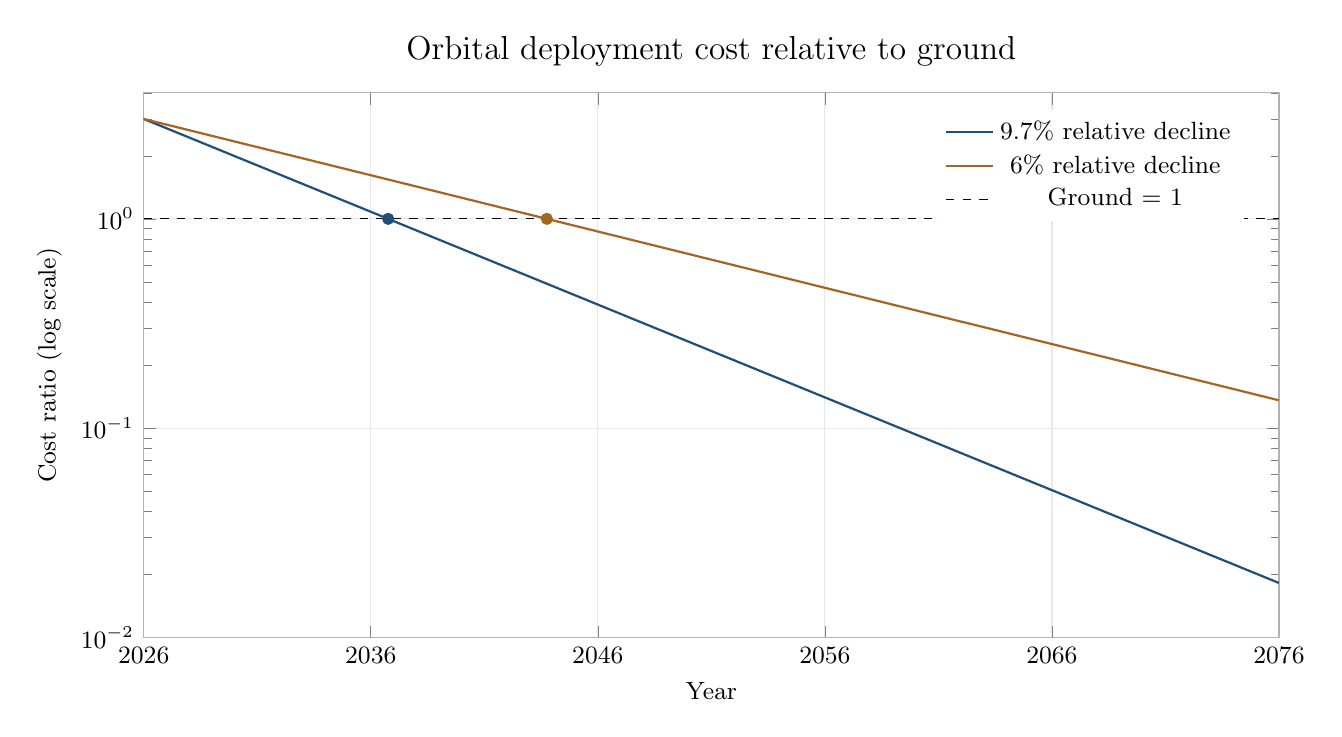
\begin{tikzpicture}\begin{semilogyaxis}[title={Orbital deployment cost relative to ground},xmin=2026,xmax=2076,ymin=0.01,ymax=4,xtick={2026,2036,2046,2056,2066,2076},xticklabel style={/pgf/number format/1000 sep={}},xlabel={Year},ylabel={Cost ratio (log scale)},legend pos=north east]
\addplot[navy,thick,domain=2026:2076,samples=101]{3*pow(0.903,x-2026)};\addlegendentry{9.7\% relative decline}
\addplot[gold,thick,domain=2026:2076,samples=101]{3*pow(0.94,x-2026)};\addlegendentry{6\% relative decline}
\addplot[black,dashed,domain=2026:2076]{1};\addlegendentry{Ground = 1}
\addplot[only marks,navy] coordinates{(2036.767,1)};
\addplot[only marks,gold] coordinates{(2043.755,1)};
\end{semilogyaxis}\end{tikzpicture}
\newpage
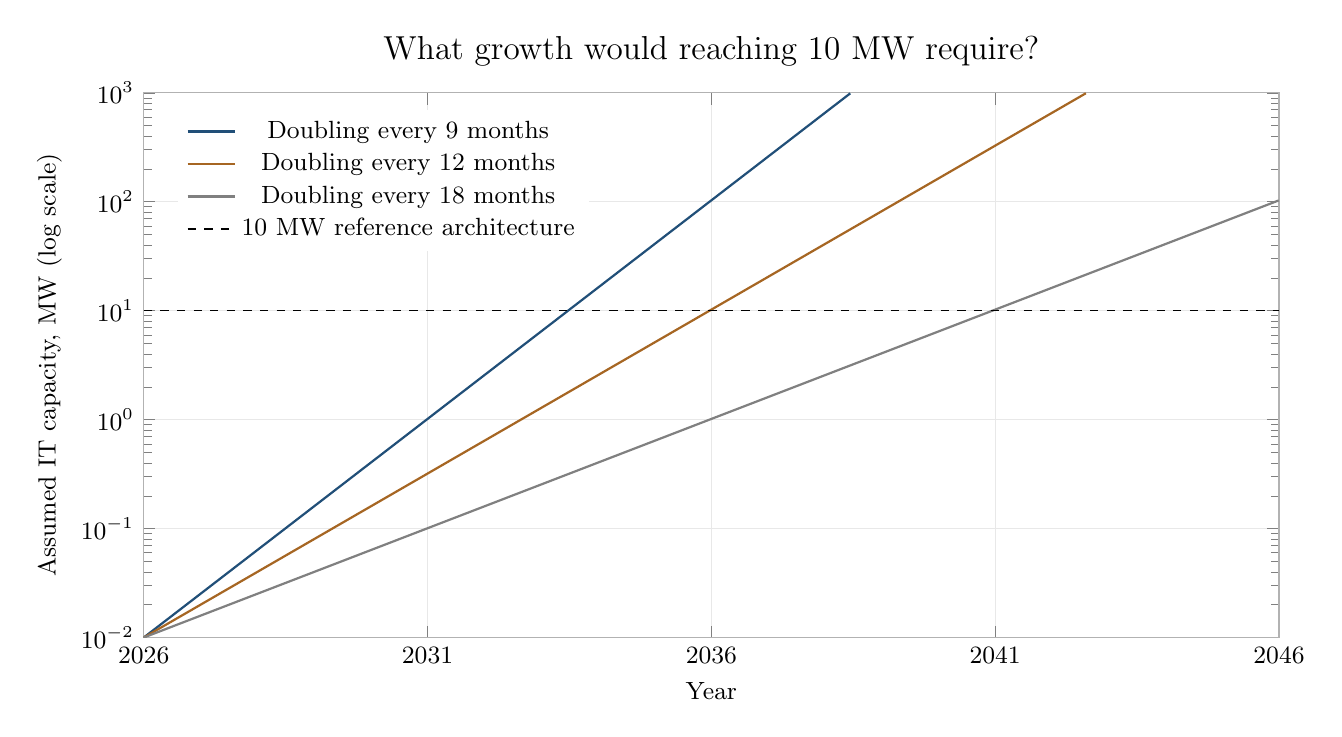
\begin{tikzpicture}\begin{semilogyaxis}[title={What growth would reaching 10 MW require?},xmin=2026,xmax=2046,ymin=.01,ymax=1000,xtick={2026,2031,2036,2041,2046},xticklabel style={/pgf/number format/1000 sep={}},xlabel={Year},ylabel={Assumed IT capacity, MW (log scale)},legend pos=north west]
\addplot[navy,thick,domain=2026:2038.45,samples=75]{.01*pow(2,(x-2026)/.75)};\addlegendentry{Doubling every 9 months}
\addplot[gold,thick,domain=2026:2042.6,samples=75]{.01*pow(2,x-2026)};\addlegendentry{Doubling every 12 months}
\addplot[gray,thick,domain=2026:2046,samples=75]{.01*pow(2,(x-2026)/1.5)};\addlegendentry{Doubling every 18 months}
\addplot[black,dashed,domain=2026:2046]{10};\addlegendentry{10 MW reference architecture}
\end{semilogyaxis}\end{tikzpicture}
\newpage
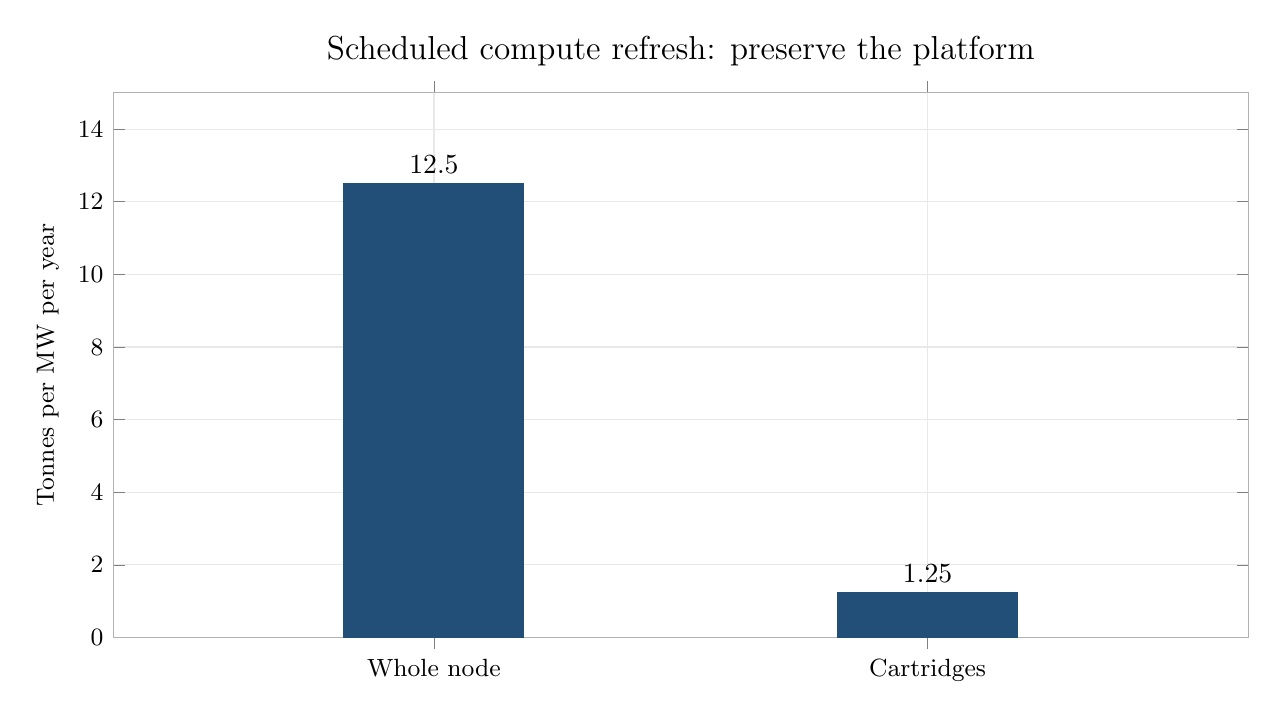
\begin{tikzpicture}\begin{axis}[title={Scheduled compute refresh: preserve the platform},ybar,bar width=65pt,ymin=0,ymax=15,symbolic x coords={Whole node,Cartridges},xtick=data,ylabel={Tonnes per MW per year},nodes near coords,point meta=y,enlarge x limits=.65]
\addplot[fill=navy,draw=navy] coordinates{(Whole node,12.5) (Cartridges,1.25)};
\end{axis}\end{tikzpicture}
\newpage
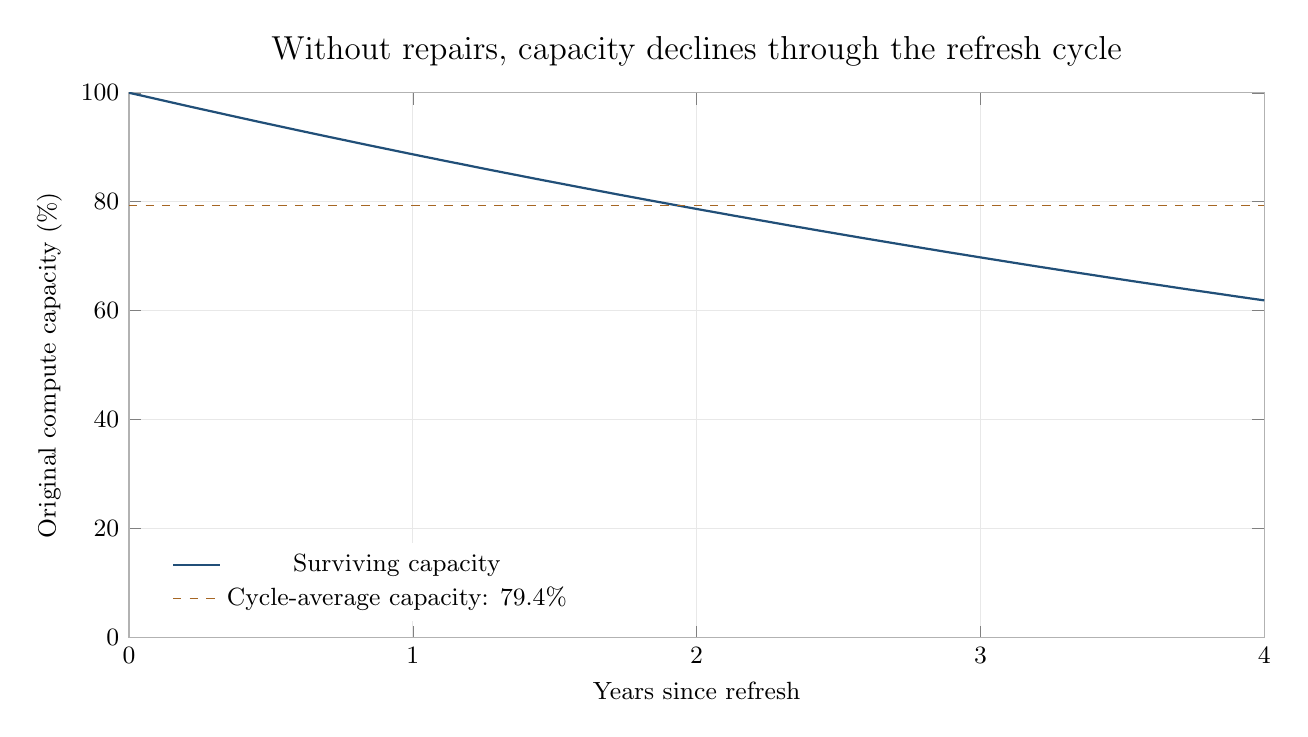
\begin{tikzpicture}\begin{axis}[title={Without repairs, capacity declines through the refresh cycle},xmin=0,xmax=4,ymin=0,ymax=100,xtick={0,1,2,3,4},xlabel={Years since refresh},ylabel={Original compute capacity (\%)},legend pos=south west]
\addplot[navy,thick,domain=0:4,samples=80]{100*exp(-.12*x)};\addlegendentry{Surviving capacity}
\addplot[gold,dashed,domain=0:4]{100*(1-exp(-.48))/.48};\addlegendentry{Cycle-average capacity: 79.4\%}
\end{axis}\end{tikzpicture}
\newpage
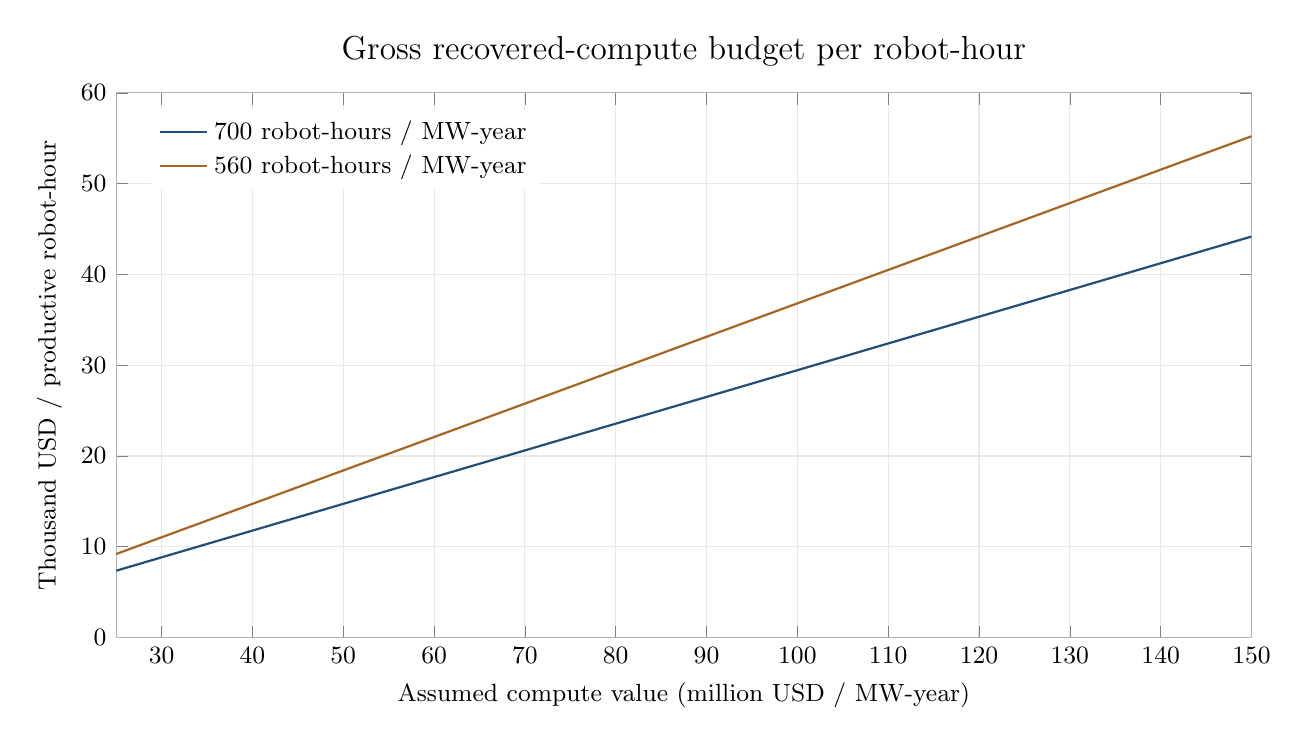
\begin{tikzpicture}\begin{axis}[title={Gross recovered-compute budget per robot-hour},xmin=25,xmax=150,ymin=0,ymax=60,xlabel={Assumed compute value (million USD / MW-year)},ylabel={Thousand USD / productive robot-hour},legend pos=north west]
\addplot[navy,thick,domain=25:150]{(1-(1-exp(-.48))/.48)*x*1000/700};\addlegendentry{700 robot-hours / MW-year}
\addplot[gold,thick,domain=25:150]{(1-(1-exp(-.48))/.48)*x*1000/560};\addlegendentry{560 robot-hours / MW-year}
\end{axis}\end{tikzpicture}
\end{document}
